\documentclass{article}
\usepackage[utf8]{inputenc}
\usepackage[french]{babel}
\usepackage[legalpaper, portrait, margin=1in]{geometry}
\usepackage{setspace}
\onehalfspacing
\usepackage{parskip}
\setlength{\parindent}{0cm}
\usepackage{enumitem}
\setlist{nosep}
\usepackage{hyperref}
\usepackage{graphicx}
\usepackage[T1]{fontenc}

\hypersetup{
  	colorlinks,
	citecolor=black,
	filecolor=black,
	linkcolor=black,
	urlcolor=black
}
\title{%
  Olympus DAO Manifesto \\
  \large DAO fonctionnel pour les projets Open Source de crypto-monnaie.}
\author{
  Berrueta, Enrique\\
  \texttt{eabz@polispay.org}
  \and
  Bustos, Ricardo\\
  \texttt{eros@polispay.org}
}
\date{Juin 2020}

\begin{document}

\maketitle

	\begin{abstract}
    Un DAO est une ``Organisation Autonome Décentralisée`` ou une société sans autorité centrale qui peut être gouvernée par une multipartie de membres autorisés choisis par une communauté plus large. Au fil des ans, plusieurs tentatives de DAO et de gouvernance ont été faites depuis le début des crypto-monnaies. Du Dash à l'Ethereum, toutes ces organisations ont connu divers problèmes, allant du manque d'organisation à la centralisation pure et simple. Après réflexion, je suis venu proposer une nouvelle solution pour créer un DAO fonctionnel, qui ne sera pas seulement décentralisé mais aussi organisé et inclusif.
	\end{abstract}

\newpage

\tableofcontents


\newpage

\section{Structure}

Le DAO sera basé sur cinq piliers fondamentaux, dont un responsable choisi par la communauté pour chaque pilier :

\begin{itemize}
  \item Technologie.
  \item Communauté.
  \item Affaires.
  \item Adoption.
  \item Marketing.
\end{itemize}

\begin{figure}[h]
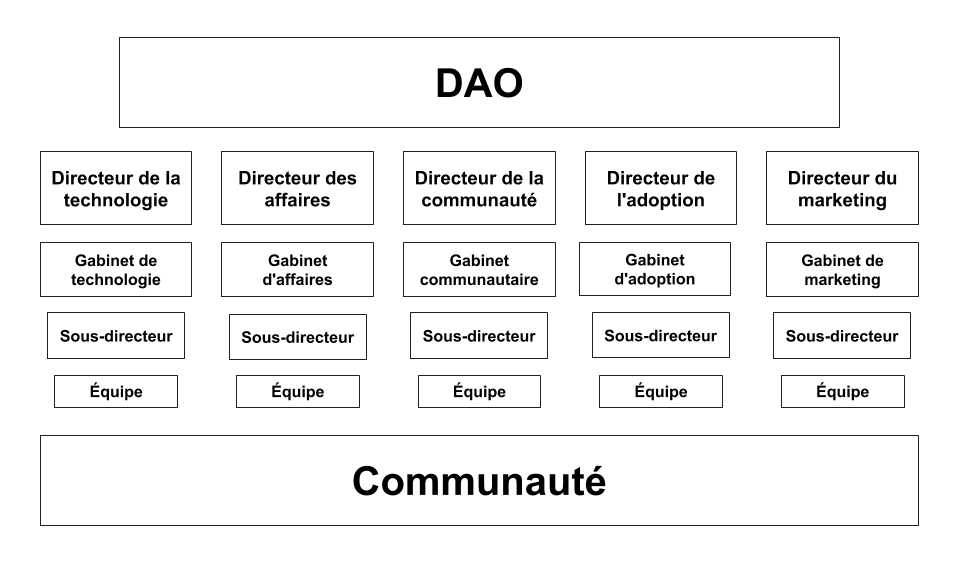
\includegraphics[scale=0.4]{img/dao_structure_fr.png}
\centering
\caption{Modèle d'organisation basique du DAO}
\end{figure}

Chaque responsable, qui s'appellera désormais ``directeur``, sera éligible en fonction de son prestige au sein de la communauté. Ils présenteront une proposition à la communauté, en précisant leurs propositions pour le cycle de commandement, qui durera un an.

Sur sa proposition, chaque directeur devra déterminer les points suivants :

\begin{itemize}
  \item Propositions d'amélioration.
  \item Les membres de leur équipe (cabinet).
  \item Les stratégies qu'ils utiliseront pour réaliser leurs propositions.
  \item Pourquoi la communauté devrait-elle voter pour eux.
  \item Feuille de route détaillée avec des calendriers spécifiques établis.
\end{itemize}

Les directeurs seront rééligibles autant de fois qu'ils le souhaitent, à condition que la communauté soit d'accord avec eux.

\section{Clés}

Comme l'ensemble du DAO est considéré comme un écosystème de crypto-monnaie, tout ce qui concerne le vote et la prise de décision doit être fait à l'aide d'une clé DAO. Ces clés sont sécurisées par le directeur et l'accès est accordé/supprimé pendant les cycles de vote du DAO ou l'exécution d'un mécanisme de sécurité.

Ces clés sont modifiées au cours des cycles de DAO si un poste de directeur change lors d'un cycle de vote ou d'un mécanisme de sécurité. Cette clé sera le récepteur des pièces pour le secteur spécifique et sera utilisée pour déverrouiller les pièces (avec les 5 autres directeurs) sur les propositions communautaires et le dépassement de budget.

\section{Plateforme}

La plateforme pour interagir, voter, proposer au DAO est la Olympus blockchain.

Tout utilisateur peut consulter les informations du DAO en temps réel, vérifiées par un nœud complet. 

Le portefeuille Olympus est la principale plateforme que les utilisateurs devraient utiliser quotidiennement pour les fonctions du DAO.

\section{Trésorerie}

Pour qu'un DAO puisse fonctionner correctement en tant qu'organisation, il est absolument nécessaire de disposer de fonds. Comme il n'est pas possible de le soutenir par des dons, nous proposons ici un modèle de financement qui garantit un financement équitable et un modèle de distribution pour chaque secteur.

Les 20\% des pièces émises chaque mois seront bloqués sur un compte utilisé pour le DAO.

Ces fonds seront répartis en trois catégories :

\begin{itemize}
  \item 10\% dans les secteurs DAO.
  \item 5\% pour les propositions communautaires.
  \item 5\% bloqué pour les secteurs qui dépassent le budget.
\end{itemize}

Le budget des secteurs du DAO sera réparti selon les proportions suivantes :

\begin{itemize}
  \item 30\% Technologie.
  \item 10\% Communauté.
  \item 20\% Affaires.
  \item 20\% Marketing.
  \item 20\% Adoption.
\end{itemize}

Les 5\% pour les propositions communautaires doivent être distribués sur la base de la décision du directeur. Ce sont eux qui décident quand une proposition doit être financée.

Les 5\% de dépassement du budget doivent être utilisés sur la base de la décision du directeur d'augmenter le budget d'un secteur spécifique pour une période spécifique.

Les fonds seront déposés automatiquement chaque mois sur la clé du directeur actuel par le réseau.

Les montants des propositions communautaires et des dépassements de budget seront déposés dans une clé à signatures multiples afin de s'assurer que seuls 3 directeurs sur 5 sont en mesure de retirer ces fonds.

Les propositions communautaires doivent être détaillées :

\begin{itemize}
  \item Montant du budget requis.
  \item Plan d'action.
  \item Budget détaillé des coûts.
\end{itemize}

\section{Cycles}

La fonctionnalité du DAO est déterminée par des cycles temporels. Il n'y a que trois cycles qui impliquent des décisions à des moments différents.

\subsection{Cycle de vote}

Le cycle de vote commence chaque année le 20 janvier. Ce processus dure environ 2 ou 3 semaines et l'idée est de faire une campagne électorale sur laquelle les anciens dirigeants et les nouveaux membres qui veulent s'impliquer techniquement auprès du DAO doivent faire leurs propositions et feuilles de route pour être qualifiés.

Ce cycle comporte quatre phases :

\begin{itemize}
  \item Postulations des candidats.
  \item Propositions des candidats.
  \item Préparation des élections.
  \item Vote.
\end{itemize}

\subsection{Cycle budgétaire}

Une fois que les directeurs sont choisis, ils doivent fournir un budget adéquat sur lequel ils fonctionneront pendant les trois prochains mois. Ce budget doit être présenté par le chef d'entreprise tous les trois mois, y compris le budget et les dépenses réelles, afin de fournir à la communauté des informations transparentes.

\subsection{Cycle des rapports}

Parallèlement aux cycles budgétaires, chaque directeur doit créer un rapport sur ses propres domaines sur les réalisations des 3 mois de travail aux directeurs et à la Communauté.

Si un directeur ne télécharge pas le rapport sur le réseau, sa clé sera automatiquement retirée des clés du DAO.

\section{Secteurs}

\subsection{Technologie}

Le responsable de la technologie sera chargé de recruter et de former des développeurs pour suivre la feuille de route technique du DAO.

Le directeur aura les fonctions suivantes :

\begin{itemize}
  \item Développement de la technologie des crypto-monnaies.
  \item Développement de cas d'utilisation.
  \item Bibliothèques tierces.
  \item Documentation et maintenance.
\end{itemize}

Aux côtés du directeur communautaire, il est chargé de la bonne fonctionnalité et de la documentation des services suivants :

\begin{itemize}
  \item Les explorateurs officiels du bloc.
  \item Sites web.
  \item Guides.
  \item Forums.
  \item Ressources internes.
\end{itemize}

\subsection{Communauté}

Le directeur en charge de la communauté sera responsable de la communauté et de l'intégrité et de l'exactitude des informations affichées sur les multiples canaux.

Le directeur aura les fonctions suivantes :

\begin{itemize}
  \item Communication et médias sociaux.
  \item Documentation et maintenance.
  \item L'assistance technique aux utilisateurs et les meilleures pratiques de sécurité.
  \item Une image de marque et design corrects.
\end{itemize}

Aux côtés du directeur de la technologie, il est responsable de la bonne fonctionnalité et de la documentation des services suivants :

\begin{itemize}
  \item Les explorateurs officiels du bloc.
  \item Sites web.
  \item Guides.
  \item Forums.
  \item Ressources internes.
\end{itemize}


\subsection{Affaires}

Le directeur responsable des affaires est chargé d'établir de nouveaux partenariats avec d'autres projets et de suivre les propositions de la communauté.

Le directeur aura les fonctions suivantes :

\begin{itemize}
  \item Partenariats.
  \item Administration et transparence budgétaire.
  \item Suivi des propositions communautaires.
\end{itemize}

\subsection{Adoption}

Le directeur chargé de l'adoption sera responsable de faire participer les commerçants au projet ainsi que d'amener les nouveaux développeurs à utiliser la technologie à leurs fins et à organiser des événements pour attirer l'utilisation du réseau.

Le directeur aura les fonctions suivantes :

\begin{itemize}
  \item Adoption des commerçants.
  \item Adoption des développeurs.
  \item Bureau des relations publiques et de l'information.
\end{itemize}

\subsection{Marketing}

Le directeur en charge du marketing sera chargé de rechercher des espaces de diffusion à condition d'amener les autres directeurs avec des stratégies analytiques et marketing.

Le directeur aura les fonctions suivantes :

\begin{itemize}
  \item Lignes de stratégies marketing et feuilles de route.
  \item Rapports d'analyse et de renseignement.
  \item Espaces publicitaires.
\end{itemize}

\section{Mécanismes de sécurité}

Comme le DAO implique de confier l'organisation à des membres connus, des mécanismes de sécurité devraient être développés sur la base de la discussion et de la sécurité du réseau.

Nous n'avons envisagé que deux cas possibles pour lesquels un problème de structure ou de fonds du DAO peut survenir. Pour couvrir ces cas, nous avons construit le mécanisme de sécurité suivant.

\subsection{Directeur de bannissement}

Si, dans quelque circonstance que ce soit, les directeurs veulent retirer un membre, ils peuvent utiliser leur clé DAO pour créer un message signé au réseau pour le retrait de la clé des clés DAO. Pour que ce mécanisme puisse fonctionner, il faut au moins 3 signatures possibles sur 5.

\subsection{Bannissement de DAO}

Ce mécanisme est exécuté par la communauté, il implique que d'une manière ou d'une autre les directeurs ne font pas leur travail correctement ou que l'ensemble du DAO est pris par un groupe qui nuit à l'ensemble de l'écosystème.

Les membres de la communauté peuvent créer un message signé avec une preuve de possession d'un certain nombre de pièces, une fois que le seuil a dépassé les 30\% de l'approvisionnement total en pièces, toutes les clés du DAO sont retirées et un cycle de vote d'urgence commence.

\end{document}
